\documentclass[aps,pre,twocolumn,letterpaper,floatfix,nofootinbib]{revtex4}
	% for \code color
\usepackage[dvipsnames]{xcolor}
\usepackage{graphicx} 
\usepackage{amsmath,amssymb,amsfonts} 
\usepackage{mathtools}
\usepackage{pdfpages}
\usepackage{afterpage}
\usepackage[hidelinks]{hyperref} 
\usepackage{epstopdf}
\usepackage{todonotes}
\usepackage{menukeys}
\usepackage{siunitx}
\usepackage{listings}
% Pretty formating of c++ (see \cpp command)
\usepackage{xspace}
\newcommand*{\cpp}{C\ensuremath{++}\xspace}

\lstdefinelanguage{LAMMPS}{
    morekeywords={units,atom_style,lattice,region,create_box,create_atoms,pair_style,pair_coeff,neigh_modify,mass,velocity,fix,run, group every, equal, count, porosity, EDGE},
    sensitive=false, % keywords are not case-sensitive
    morecomment=[l]{//}, % l is for line comment
    morecomment=[s]{/*}{*/}, % s is for start and end delimiter
    morestring=[b]" % defines that strings are enclosed in double quotes
}

\lstset{
numbers=left, 
numberstyle=\small, 
numbersep=8pt, 
frame = single, 
language=LAMMPS, 
framexleftmargin=15pt,
xleftmargin=0.65cm,
xrightmargin=0.1cm}

% Highlighte inline code
\definecolor{light-gray}{gray}{0.95}
\definecolor{atomify-red}{rgb}{0.90196078 , 0.09803922, 0.29411765}
\definecolor{atomify-green}{rgb}{0.23529412 , 0.70588235, 0.29411765}
\definecolor{atomify-yellow}{rgb}{0.8,  0.70588235,  0.07843138}
\definecolor{atomify-blue}{rgb}{0.00000000 , 0.50980392, 0.78431373}
%\newcommand{\code}[1]{\mbox {\texttt{#1}}}
\newcommand{\code}[1]{\colorbox{light-gray}{\color{RawSienna}\texttt{#1}}}

\begin{document}

\title{Increased productivity using Atomify - a real-time LAMMPS visualizer}
\author{Anders Hafreager$^1$}
\author{Svenn-Arne Dragly$^{1}$} 
\author{Anders Malthe-S\o renssen$^1$}
\affiliation{$^1$Department of Physics - University of Oslo\\Sem S{\ae}lands vei 24, NO-0316, Oslo, Norway }
\date{\today} 

%%%%%%%%%%%%%%%%%%%%%%%%%%%%%%%%%%%%%%%%%%%%%%%%%%%%%%%%%%%%%
%%%%%%%%%%%%%%%%%%%%%%%%%%%%%%%%%%%%%%%%%%%%%%%%%%%%%%%%%%%%%

\begin{abstract}
%
The typical workflow when running atomistic simulations includes working with several programs.
A text editor is needed to create and modify the scripts, the terminal to run the simulation, and programs like VMD or Ovito to visualize the system over time.
If physical quantities are computed, the data is often plotted with MATLAB or Python, where additional scripts must be used.
This is a tedious process, especially for teaching purposes and for people who are new in the field.
We here introduce Atomify; a high performance real-time visualizer for atomistic simulations that can simulate and render more than one million atoms with excellent frame rate on modern hardware.
Atomify supports OpenMP acceleration, GPU acceleration, real-time plotting of physical quantities, and an easy-to-use code editor in one single application.
It currently uses LAMMPS as physics engine, but it can be extended to support other codes like Gromacs, NAMD or OpenMM.
Atomify is open-source software (GPL) written in C++ using the Qt framework.
%
\end{abstract} 
 
\maketitle

\section{Introduction}
Our nature is a very complex system with complicated rules that determine how, and where mass, energy and momentum is transferred.
Many macroscopic observable effects result from microscopic details on the atomic level such as melting of ice, and even life.
Understanding the world from a bottom-up perspective requires us to be able to model a physical system from the atomic scale where the timescale is of order femtoseconds.
Many physical and chemical processes happen on nanosecond timescales, some even during a few picoseconds, which means thousands or millions of timesteps of \SI{1}{\femto\second} need to be calculated.
Much has happened since the first molecular dynamics simulation of hard spheres in the 1950s\citep{alder1957phase,alder1959studies}, and later, in 1964, a more realistic system with the Lennard Jones potential studying diffusion in argon\citep{rahman1964correlations}.
The computing power has seen a tremendous increase from the CDC 3600 used in \citep{rahman1964correlations}, which performed less than 1 million instructions per second whereas modern 3 Ghz processors in typical laptops can do about 100 billion instructions per seconds.
With this rapidly increase of computing power, the lengthscales and timescales achievable in numeriments\footnote{Numeriment is a numerical experiment, or a simulation on the computer.} is finally catching up with some experiments (ref).

In molecular dynamics, a set of atoms is integrated using Newton's second law in a classical force field so the full coordinate in the phase space is known at all times, and statistical properties can be calculated from averages assuming ergodicity\citep{martyna1994constant}.
The model has been proved successful in reproducing and explaining many phenomenon such as mechanical properties \citep{jiang2009young, campbell1999structural, ning2012mechanical}, chemical reactions \citep{van2001reaxff, brenner2002second}, liquid properties\citep{allen2017computer}.
Also in biology, molecular dynamics is useful blabla. \todo{Add more nice references here}

Over the years, increasingly sophisticated methods have been developed.
For instance, a non-equilibrium method to measure thermal conductivity using heat exchange, was recently improved\citep{wirnsberger2015enhanced} to conserve energy better than the previous method\citep{ikeshoji1994non}.
To study first order phase transitions, methods like the generalized replica exchange method (gREM)\citep{kim2010generalized} can be used, and nudge elastic band (NEB)\citep{henkelman2000climbing, henkelman2000improved} is often used to study energy barriers in for instance chemical reactions.
In addition, a huge amount of force fields exists, each being good at different properties\footnote{Some force fields are good at reproducing mechanical properties while others may be good at chemical reactions. This usually depends on what properties the force field was fitted to.}.
New hardware and a sea of optimization tricks makes implementing a good molecular dynamics code a challenging task, not to mention maintaining it over time when new arcitechtures are being released.
Each new feature or technique may take days, if not weeks, to develop, preventing researchers to work on their scientific projects.

Thankfully, there already exists several software packages for atomistic simulations, many of which have been developed for more than two decades\footnote{\url{https://en.wikipedia.org/wiki/Comparison_of_software_for_molecular_mechanics_modeling} compares different softwares for molecular modeling.}.
Some of these packages, such as LAMMPS\citep{Plimpton1995Fast}, Gromacs\citep{berendsen1995gromacs}, NAMD\citep{Phillips2005Scalable} and CHARMM\citep{brooks2009charmm}, are open source and being actively developed with hundreds of contributers\footnote{See their repositories on i.e. GitHub for an overview of contributers.}.
%After the rise of powerful graphical processing units (GPU's), most of these codes eventually added support of using accelerators\citep{brown2011implementing}.

\lstinputlisting[language=LAMMPS,caption={A minimal LAMMPS input script that simulates a Lennard Jones solid at reduced temperature $T^* = 1.0$ with a reduced density of $\rho^* = 0.8442$.},label={lst:simple.in}]{simple.in}

The work in this paper is focused on LAMMPS.
Although the software is well-documented\footnote{The LAMMPS documentation is known for being very detailed and precise.}, and enables the user to perform advanced simulations, it can be a demanding task to learn how to use it well.
The core principles of molecular dynamics is so simple that high school students can easily understand the concepts, but even undergraduate students may have problems with the terminology of statistical mechanics which is used in several of the commands.
For instance, to simulate an \textit{NVE} simulation (constant number of particles $N$, volume $V$ and energy $E$), we use the \code{fix nve} command which defines the time integration.

A LAMMPS simulation is performed by a series of commands, which are executed one by one.
LAMMPS has a huge list of implemented features which makes it very flexible, especially with its own, powerful scripting language.
In listing \ref{lst:simple.in}, we show an example of a minimalistic LAMMPS script that simulates 4000 Lennard Jones atoms in an FCC lattice with reduced temperature $T^*=1.0$ and reduced density $\rho^* = 0.8442$.
This simulation does not print much thermodynamic data, but it creates a file \code{trajectory.bin} which containes the trajectory of all atoms at every timestep.
Other programs such as VMD\citep{Humphrey1996Vmd} or OVITO\citep{Stukowski2009Visualization} can be used to visualize the file as a postprocessing step.

If we want to measure physical quantities such as energy, temperature and stress, they can be accessed through commands called \textit{computes}.
For instance, the commands \code{compute ke} and \code{compute pe} measures the kinetic and the potential energy.
Using \textit{fixes}, we can create time averages and save them to one or more files for plotting and further analysis.
We also often put atoms in different \textit{groups}, either by their position being in a \textit{region}, or their atom type or more advanced criteria.
Performing different operations on different groups, or just measuring physical quantities on a specific group is then easily done since almost all commands have \code{group} as an input parameter.
With this flexibility, it may be difficult to do everything right immediately.
Complicated regions and group defines are often necessary to perform the intended simulation, and a lot of time can be spent in the prototyping process, especially since information about groups and regions are not automatically written to a trajectory file.
A simulation typically involves writing the LAMMPS script in a text editor before the simulation is performed in the terminal for a while before the trajectories and time series are studied to verify the correctness which often turn out to be bad.
Plotting of time series also requires the user to write a script in i.e. Python or MATLAB which does the plotting, but these steps are often performed manually.

\begin{figure*}
	\centering
	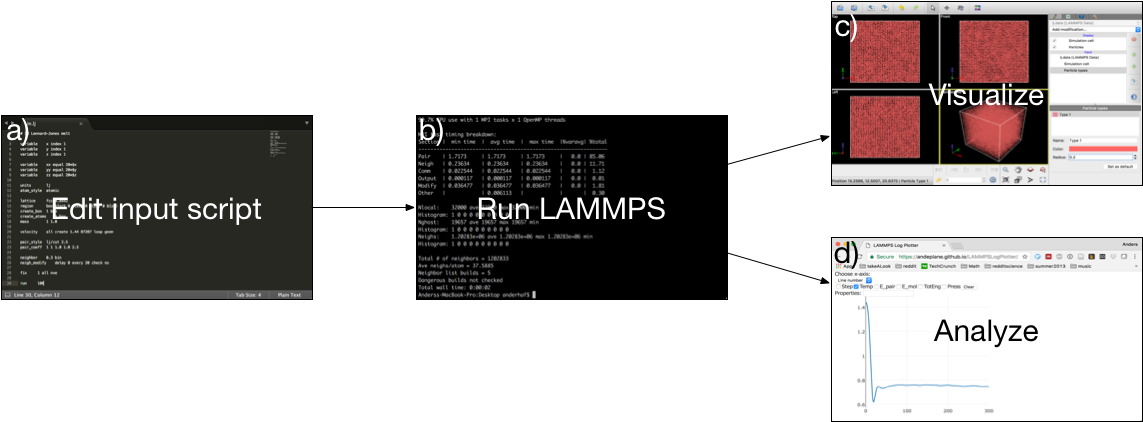
\includegraphics[width=0.95\textwidth]{flowchart.png}
	\caption{The typical workflow when using LAMMPS consists of multiple steps using several applications.
	a) A LAMMPS script is written using a text editor.
	b) Simulation is performed from the terminal.
	c) and d) visualization and analysis is performed using Ovito and \url{http://bit.ly/logplotter}.
	Atomify simplifies the workflow by combining all steps into a single application.}
	\label{fig:flowchart}
\end{figure*}

The lack of an intuitive GUI and visualization\footnote{GUI is listed as a non-feature on the LAMMPS web page: \url{http://lammps.sandia.gov/non_features.html}.}
makes this workflow complicated, see Fig. \ref{fig:flowchart}.
The time from an idea to a visual feedback can then be destructive for the creativity where immediate feedback would be ideal.

We have solved this problem by creating Atomify, a real-time LAMMPS visualizer that combines script editing, simulation, visualization, and analysis in one single application.
It uses LAMMPS as a library and hooks into the LAMMPS simulation cycle so synchronization of atom positions and physical quantities can be performed as often as every timestep.
Most features of LAMMPS are automatically supported, except a few due to technical reasons discussed in section \ref{sec:future}.

The visualization is performed using the powerful Qt3D library where we have implemented advanced rendering techniques such as billboard raytracing to achieve maximum performance.
This allows visualization of millions of atoms with good framerate on modern desktop computers.
Atomify is designed with simplicity as its main goal.

Since we have used the Qt framework to develop Atomify, and LAMMPS is written in object oriented \cpp, a simplified version is also made available on mobile platforms (Android and iOS).
This version of Atomify provides access to some of the example simulations and is intended for exploration of molecular dynamics simulations by students and scientific outreach.
It also works as a demonstration of the visualization capabilities of the desktop version of the software.
The authors are optimistic that teachers can use the visualizations provided by
Atomify to explain microscopic interactions underlying concepts in topics such
as thermodynamics, geophysics, and biology.

\begin{figure*}
	\centering
	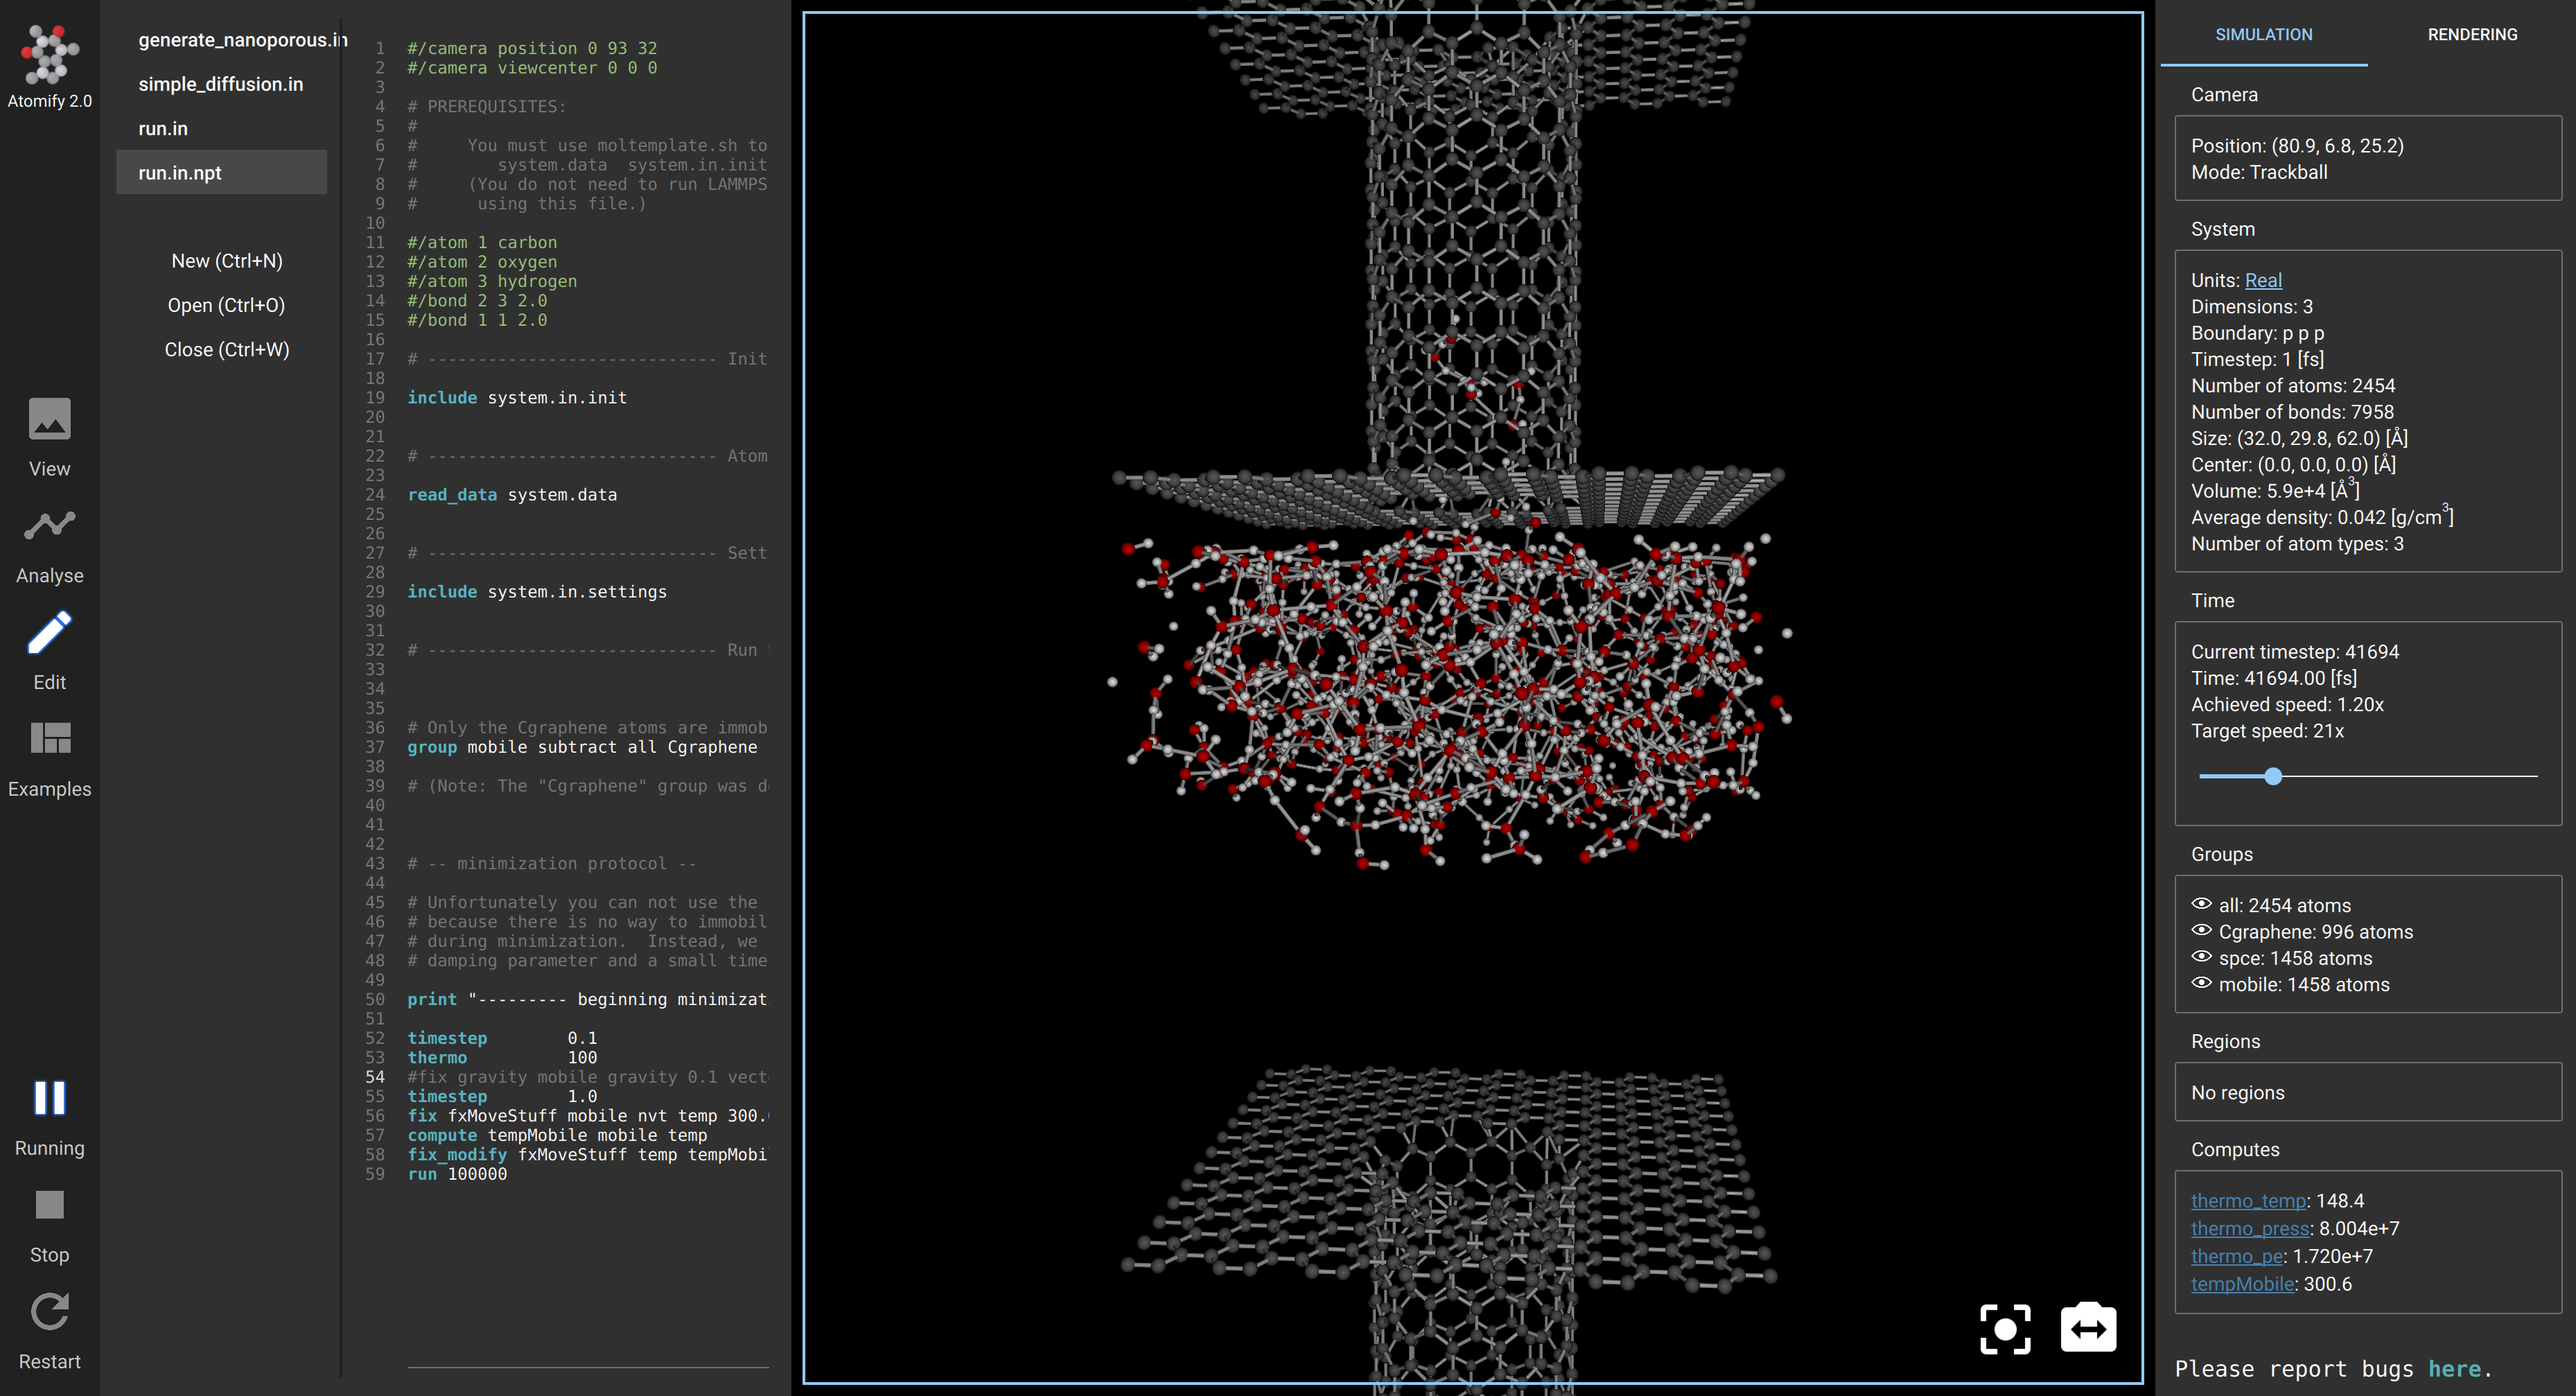
\includegraphics[width=\textwidth]{gui.png}
	\caption{%
    Overview of the Graphical User Interface (GUI) in Atomify.
    The toolbar (1) is used to change between the different modes, such as 
    editing, viewing and analyzing the running simulation, 
    in addition to playback controls.
    The file browser (2) contain the list of open LAMMPS scripts or data files.
    The text editor (3) provides code highlighting.
    The viewport (4) shows the current simulation.
    The simulation properties (5) shows the simulations details, gives access to 
    LAMMPS objects such as groups, regions and computes, and the rendering
    properties (6) lets you change the viewport settings, such as lighting and
    draw mode.
    TODO: Add numbers to figure.
    }
	\label{fig:gui}
\end{figure*}

In this paper we will go through a case study, an example simulation, where we
use many of the useful features Atomify provides.
We start by discussing the GUI in section \ref{sec:features} where the main features are summarized.
In section \ref{sec:casestudy}, the case study is introduced where we go through a typical example
of a simulation that uses regions and groups to perform different integration on different atoms.
Common pitfalls which are easily picked up with Atomify are shown.
Details about how Atomify runs LAMMPS is found in section \ref{sec:implementation} where the data flow and the threading model is explained.
Finally, we summarize the work in our paper in section \ref{sec:conclusion} with some thoughts about future outlooks in section \ref{sec:future}.

\section{\label{sec:features}Summary of features}
The main features of Atomify can be summarized as script editing,
real-time visualization and plotting of physical quantities.
This turns out to improve the workflow substantially.
In addition, Atomify comes with multiple examples,
many of which have been made by members of the LAMMPS community.

\begin{figure}
	\centering
	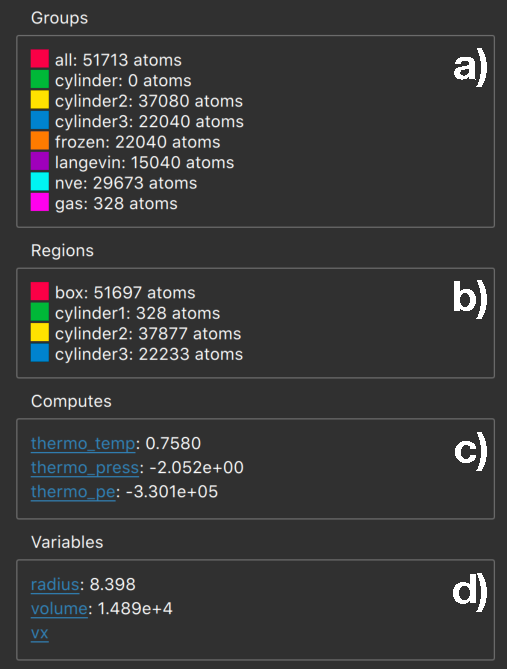
\includegraphics[width=0.5\textwidth]{figures/rightbar.pdf}
	\caption{
		The rightbar is a powerful feature in Atomify where relevant
		properties from LAMMPS is presented real-time.
		In a), a list of all groups defined is shown with the current atom count.
		b) shows all defined regions. Each group and region can be hovered so that atoms
		are colored after what group / region they are in. If an atom is in multiple
		groups or regions, they will get the color of the latest one defined.
		The color boxes can be clicked which will either always highlight the atoms in a certain group or region,
		or if clicked again, hide all of them.
		In c) and d), a list of all variables and computes is shown. If a variable or compute
		produces a scalar, the current value is shown as can be seen with all the variables.
		By clicking the name, a plot will show up showing the time evolution of that quantity.
		If a per-atom variable or compute is hovered, all atoms will be colored according to their
		current scalar value and a histogram over these values is shown if clicked.
		The result of hovering atoms defined by the groups in our case study is shown in Fig. \ref{fig:cylinder_simulation}.
    }
	\label{fig:rightbar}
\end{figure}

It provides a lightweight script editor with syntax highlighting and line numbers.
Multiple files can be open at the same time and the state persist across working sessions.
The script can easily be restarted by clicking the button in the GUI or using
the default shortcut (\keys{Ctrl+R} in Windows and Linux or \keys{\cmd+R} in macOS).
This enables the user to get immediate visual feedback on changes in the script.

\section{\label{sec:casestudy}Case study: flow through nanoporous media}
The features of Atomify is best presented through a case study where many of the features are useful to be productive in the script development.
We have chosen to create a system with fluid flow inside a tight nanochannel.
This involves creating a somewhat complicated initial geometry with multiple regions where we apply different tricks such as dissipative thermostats, constant force mimicking applied pressure gradient and frozen atoms to avoid net momentum of the solid.

Fluid flow in porous media is often characterized with permeability, the inverse flow resistance of a material.
The permeability can be measured using Darcy's law when applying a pressure gradient.
However, the derivation of Darcy's law assume no-slip boundary conditions, i.e. the fluid velocity is zero at the boundary of a channel. (ref)
This is a good approximation for liquids in larger pores, but if the channel size $R$ is of the same order, or larger, as the mean free path $\lambda$ of the fluid, this is no longer true. (ref)
The Knudsen number, $\text{Kn} = \lambda / R$ quantifies this and can be used to apply Klinkenberg correction\citep{klinkenberg1941permeability} to correctly describe the effective permeability as a function of pressure in the high Knudsen number limit.

\begin{figure}
	\centering
	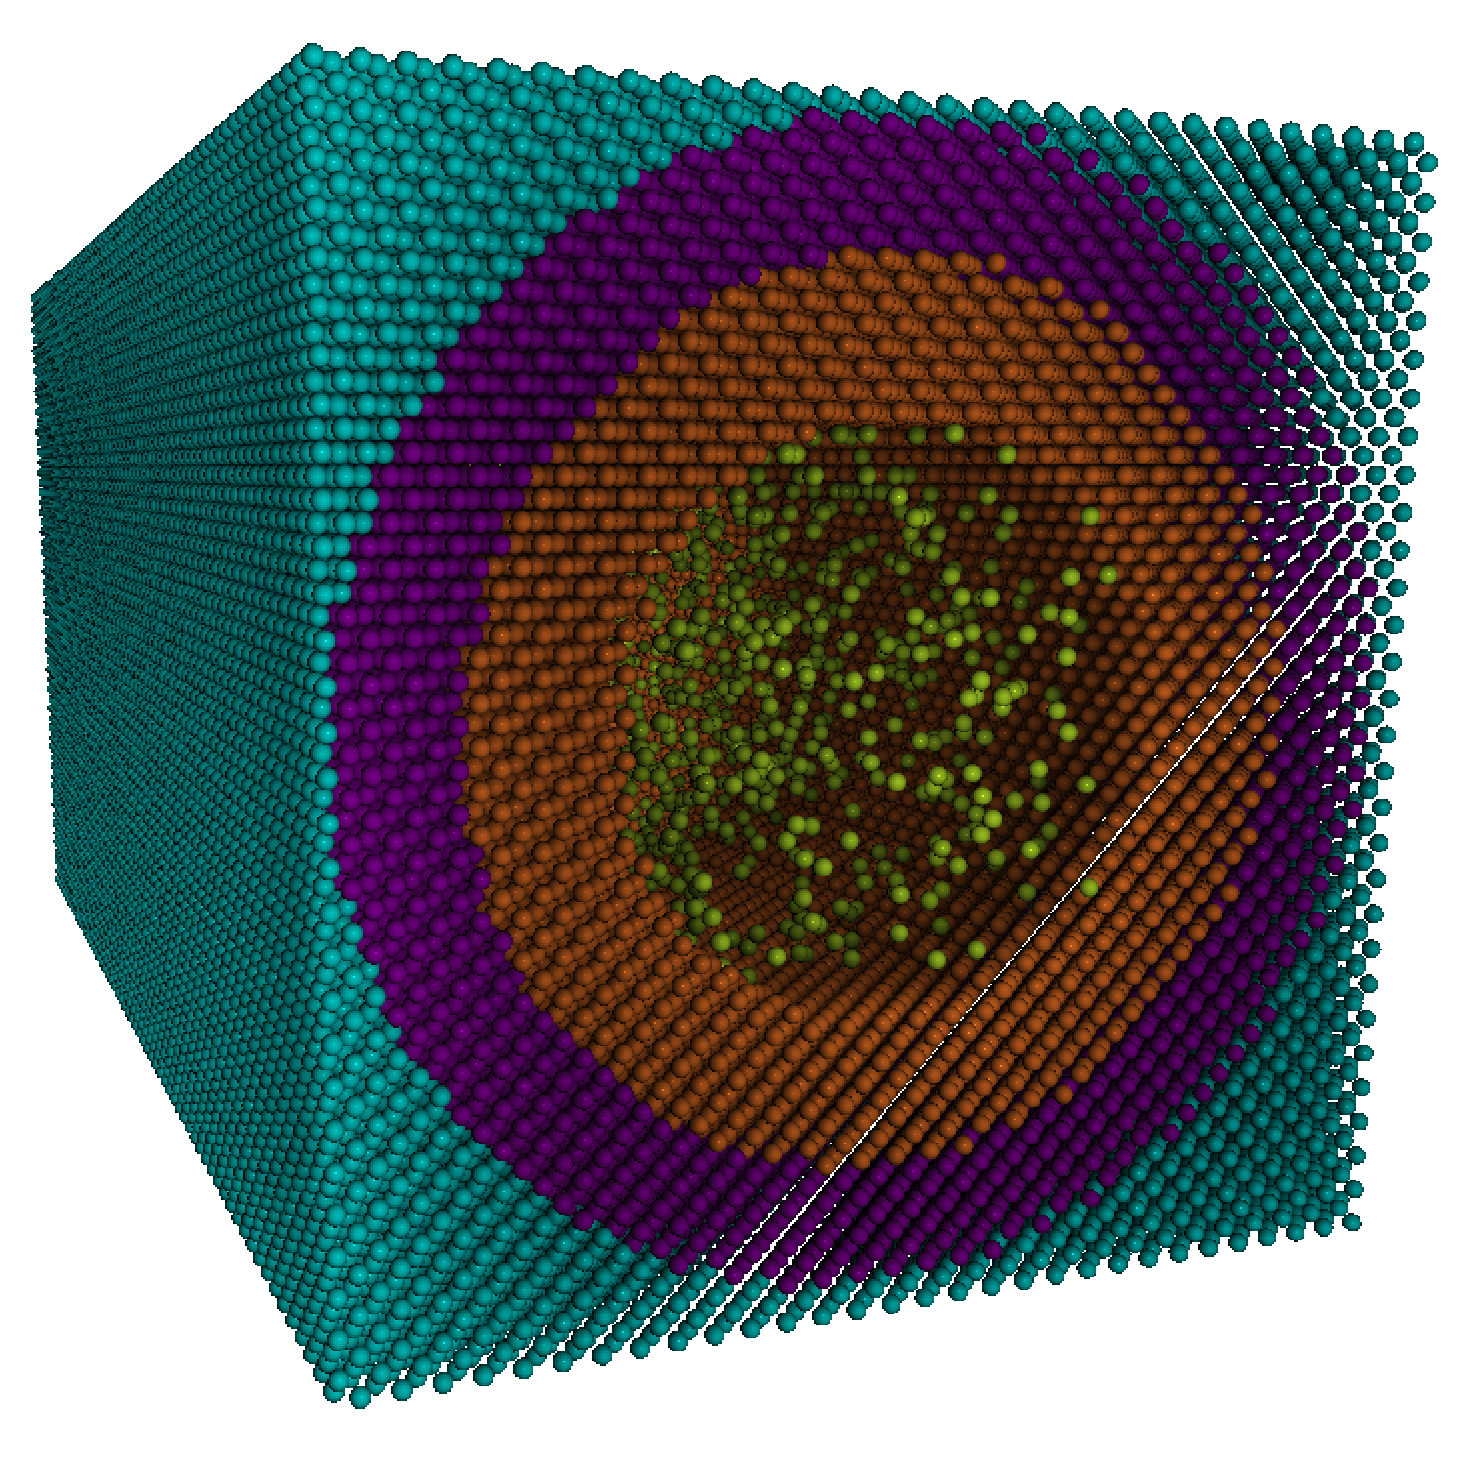
\includegraphics[width=0.5\textwidth]{lj_flow/configuration.png}
	\caption{
		Initial configuration in our case study simulation.
		A periodic box consisting of $(40\times25\times25)$ FCC unit cells with reduced density $\rho^* = 0.8442$ where we will have gas flow in a cylinder with radius 10 (reduced length).
		The different colors indicate the regions of which different integration rules apply.
		\textcolor{atomify-blue}{Blue} atoms are fixed and do not move at all,
		whereas the \textcolor{atomify-yellow}{yellow} atoms are thermalized with a Langevin\citep{schneider1978molecular} dissipative thermostat to mimick the heat exchange with the frozen bulk atoms.
		The \textcolor{atomify-red}{red} and the \textcolor{atomify-green}{green} atoms are integrated normally, except the \textcolor{atomify-green}{green} gas atoms have an applied constant acceleration representing the pressure gradient.
		Setting up and verifying this system is simple using Atomify due to the real-time coloring of groups and regions.
    }
	\label{fig:cylinder_simulation}
\end{figure}

In this case study, we will use Atomify to measure the velocity profile of a Lennard Jones gas inside a nanotube with varying density to observe the slip velocity effect at low densities.
We will create the nanotube inside a Lennard Jones solid of size  $(40\times25\times25)$ unit cells with reduced density $\rho^* = 0.8442$. The fluid in the nanochannel, or cylinder, will flow due to an induced pressure gradient, see Fig. \ref{fig:cylinder_simulation}.
Here we apply a pressure gradient $\nabla P$ in the $x$-direction on the gas atoms using a constant acceleration $a$ calculated as
\begin{align}
	a = \frac{\nabla P}{\rho_m},
\end{align}
where $\rho_m$ is the mass density of the gas atoms.
Applying such an acceleration means adding energy to the system which in turn will increase the temperature and eventually melt the system.
To avoid this, we will couple the solid to an external heat bath so the added energy can be transferred away from the system through a thermostat.
Even though we only apply a pressure gradient on the gas atoms, this induced momentum will also be transferred to the solid atoms which eventually will start moving in the positive $x$-direction which is not desired.
We therefore freeze the outmost atoms (blue in Fig \ref{fig:cylinder_simulation}).
To achieve these properties of the system, the atoms are divided into multiple regions, which are integrated differently:

\begin{itemize}  
	\item $r \leq 10$: applied pressure gradient
	\item $5 < r \leq 4$: regular time integration
	\item $9 < r \leq 12$: Dissipative Langevin thermostat
	\item $12 < r$: frozen.
\end{itemize}
The different radii are in reduced Lennard Jones units.

\subsection{Creating the initial geometry}
We create a new script in Atomify using \keys{\cmd+N}, and save it (\keys{\cmd+S}) as \code{run.in}.
Starting from the input script in listing \ref{lst:simple.in}, we modify it to create a larger simulation box with $(40\times25\times25)$ unit cells.
Remove the line \code{fix nve all nve} so atoms will stand still (we will add integrator later anyway).
We will modify this script to achieve what we described above, so we need to make sure that these commands happen \textit{before} the \code{run 1000} command in the script.
If not, LAMMPS will not execute them before we start visualizing.
To define the inner cylinder, we first specify the radius and the center before using the region command
\begin{lstlisting}[basicstyle=\tiny, frame = none, numbers=none, framexleftmargin=0pt, xleftmargin=-0.75cm, xrightmargin=0.0cm]
	variable R equal $(ly*0.25)
	variable c equal $(ly*0.5)
	region cylinder1 cylinder x $c $c $R EDGE EDGE
\end{lstlisting}
The region command will create a cylinder in the $x$-direction, with $(y,z)$-coordinates at the system center \code{\$c} with radius \code{\$R} using the full length of the cylinder specified when using \code{EDGE}.
We now press \keys{\cmd+R} to run the simulation to see how it looks.
As shown in Fig. \ref{fig:rightbar}, we can hover the specified region to highlight the atoms in that region.
When we hover the region, we immediately see that the cylinder is in fact not placed at the center of the system, as shown in Fig. \ref{fig:initial_configuration}a.
The reason is that LAMMPS operate with two different units, either the length unit or the lattice length unit. This is explained in the documentation, but is a common mistake.
To discover mistakes like this is quickly done with Atomify.
Since we have used \code{\$(0.5*lx)}, we need to specify \code{units box} in the region command, rerun the simulation with \keys{\cmd+R} which gives the desired result in figure  \ref{fig:initial_configuration}b.

\begin{figure}
	\centering
	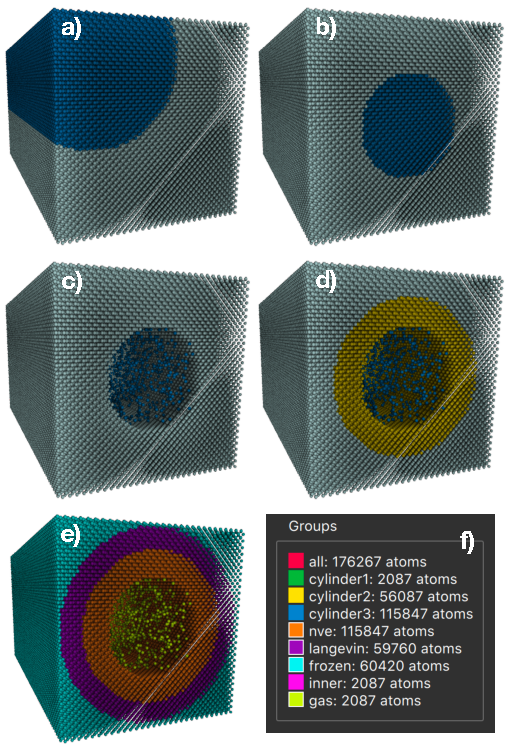
\includegraphics[width=0.5\textwidth]{figures/initial_configuration.pdf}
	\caption{
		Several snapshots of the process of creating the simulation in our case study.
		This shows how one typically generate a geometry step by step where the immediate
		feedback is very useful to quickly discover mistakes.
		The wrongly placed cylinder is shown in a) whereas it is placed correctly in b).
		c) shows how the system looks after deleting atoms to obtain $\rho = 0.01$. The next cylinder $C_2$ is shown in d),
		and all regions (placed in groups) are shown in e). Here we have uniquely defined the purple shell which should have a dissipative thermostat.
		In f), the list of all groups defined in this system is shown with colors matching those of e). All figures are rendered with Atomify.
    }
	\label{fig:initial_configuration}
\end{figure}
We now want to delete atoms so that we have a certain density. The volume of the inner cylinder is $\pi R^2 L$ which can be calculated in lammps with \code{variable V equal PI*v\_R*v\_R*lx}.
In these units, we have chosen that the atomic mass is 1 so number density $\rho$ equals the mass density $\rho_m$.
The command \code{delete\_atoms} can be used: \code{delete\_atoms porosity region-ID fraction seed}, where we need to specify the fraction of the existing atoms in that region we want to delete.
To count the number of atoms inside a region, we first create a group containing all the atoms in the region and then create a variable that counts them.
Assuming a density $\rho = 0.05$, we can calculate the expected number inside the cylinder as $N = V\rho$.
The atoms inside the region can now be deleted. These steps can be done in LAMMPS like this
\begin{lstlisting}[basicstyle=\tiny, frame = none, numbers=none, framexleftmargin=0pt, xleftmargin=-0.75cm, xrightmargin=0.0cm]
	group cylinder1 region cylinder1
	variable N_cyl equal count(cylinder1)
	variable V equal PI*v_R*v_R*lx
	variable rho equal 0.1
	variable N_wanted equal $V*${rho}
	variable delete_fraction equal (${N_cyl}-${N_wanted})/${N_cyl}
	delete_atoms porosity cylinder1 ${delete_fraction} 1234
\end{lstlisting}
and the result is shown after rerunning again with \keys{\cmd+R}, see Fig. \ref{fig:initial_configuration}c.
This is a powerful workflow Atomify enables where very quick changes can be tested with immediate feedback.
Every time we add a new command, we just rerun with \keys{\cmd+R} to see what happens.

The next step now is to create a larger cylinder, the one containing the red atoms in Fig. \ref{fig:cylinder_simulation}, where regular time integration will take place.
This cylinder should have a slightly bigger radius as stated above and can be created with another region command:
\begin{lstlisting}[basicstyle=\tiny, frame = none, numbers=none, framexleftmargin=0pt, xleftmargin=-0.75cm, xrightmargin=0.0cm]
	region cylinder2 cylinder x $c $c $(v_R+4) EDGE EDGE
\end{lstlisting}
Again press \keys{\cmd+R} and see the expected result in Fig. \ref{fig:initial_configuration}d.

Now we have the inner cylinder with the gas atoms defined as a region and the next cylinder shell (including the gas atoms) defined as another region.
We now want to create another shell, the one with the dissipative thermostat.
All the atoms with the dissipative thermostat, the inner shell and the gas will be integrated with the \code{fix nve} integrator.
Therefore, we create a slightly larger cylinder which will be the one defining the group for \code{fix nve}.
We can also define the groups with these cylinders
\begin{lstlisting}[basicstyle=\tiny, frame = none, numbers=none, framexleftmargin=0pt, xleftmargin=-0.75cm, xrightmargin=0.0cm]
	region cylinder3 cylinder x $c $c $(v_R+7) EDGE EDGE
	group cylinder1 region cylinder1
	group cylinder2 region cylinder2
	group cylinder3 region cylinder3
	group nve region cylinder3
\end{lstlisting}
where we also have created the group \code{nve} for clarity.

The dissipative thermostat will be \code{fix langevin}\citep{schneider1978molecular}, but it should only be applied on the outer shell defined by $C_3 \setminus C_2$,
where $C_i$ is the set containing the atoms inside cylinder $i$.
We can obtain this with the command

\begin{lstlisting}[basicstyle=\tiny, frame = none, numbers=none, framexleftmargin=0pt, xleftmargin=-0.75cm, xrightmargin=0.0cm]
	group langevin subtract cylinder3 cylinder2
	group frozen subtract all cylinder3
	group gas dynamic all region cylinder1 every 1
\end{lstlisting}

which will contain only the outer shell. 
We here also created the group \code{frozen}, which is the outmost atoms, and the group \code{gas} which is dynamic since atoms may switch places and we want to only apply a force on the ones in the inner cylinder at any point in time.
The frozen atoms will not move at all and make sure that the system does not start moving due to momentum transfer from the gas particles through the solid.
All these groups are highlighted in Fig. \ref{fig:initial_configuration}e by hovering the box containing all the groups. in Atomify as shown in Fig. \ref{fig:initial_configuration}f.
The colors of the atoms matches the group color next to the group name in Fig. \ref{fig:initial_configuration}f, where the order of coloring is the same as they were defined in the script.
We there don't any green atoms (\code{cylinder1}) since all of these are in the groups \code{cylinder2}, \code{cylinder3}, \code{nve} and \code{gas}.

\subsection{Physical setup}
Now that we have achieved to set up the system geometrically, that is, all the different groups of atoms are defined.
We only need to apply the different actions, or fixes, on them.
First, we apply the time integration \code{fix nve} which should happen on all atoms within $C_3$, then the thermostat \code{fix langevin}

\begin{lstlisting}[basicstyle=\tiny, frame = none, numbers=none, framexleftmargin=0pt, xleftmargin=-0.75cm, xrightmargin=0.0cm]
	fix nve nve nve
	fix langevin langevin langevin 1.0 1.0 1.0 12345
	compute displacement all displace/atom
\end{lstlisting}

The syntax for fixes is \code{fix ID groupID style args}, so the above fixes has the same name as both the groups and the fix style.
\code{fix langevin} takes at least 4 arguments \textit{Tstart, Tstop, Tdamp, seed}, i.e. the temperature in the beginning of a simulation, the temperature at the end (timesteps in between get a linearly interpolated temperature between these values), a damping parameter which controls how strongly the thermal bath interacts with the system.
It also needs a random seed due to the random nature of the Langevin thermostat, see \citep{schneider1978molecular} for details.
Finally, we have added another compute that measures the displacement per atom.
Hovering this compute in the list will color each atom according to their displacement since $t=0$.

By rerunning again (\keys{\cmd+R}), we can confirm that the system behaves as expected.
In Fig. \ref{fig:moving_atoms}, we see that the outmost atoms are completely frozen (dark blue), the ones in the solid are also blue, but brighter, since they vibrate thermally in the lattice.
The inner cylinder contains gas atoms which move more freely, as seen from the colors being in the upper part of the color map.

\begin{figure}
	\centering
	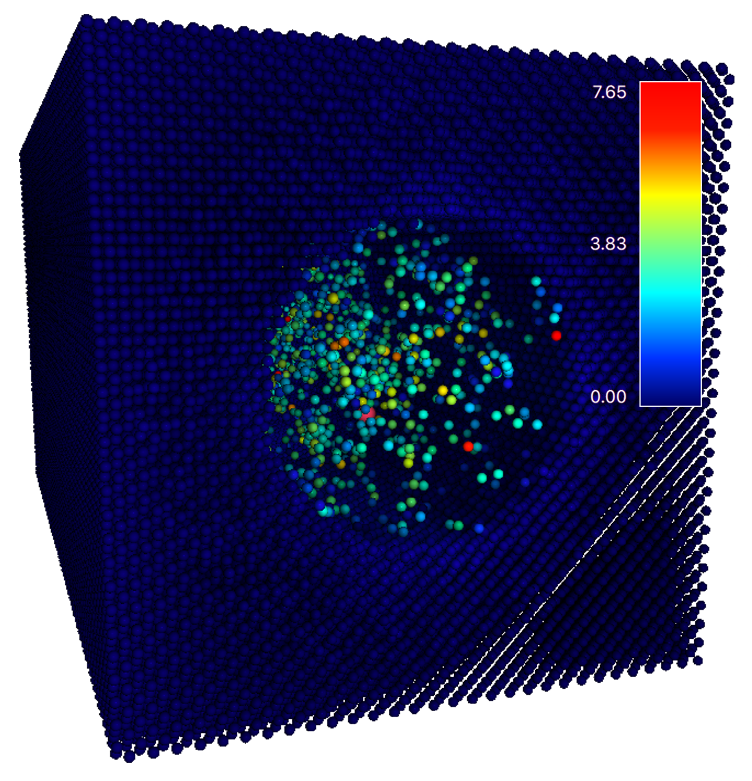
\includegraphics[width=0.5\textwidth]{lj_flow/07_moving.png}
	\caption{
		We see the expected moving atoms inside the $C_3$ cylinder.
		The atoms are colored based on their displacement (measured in reduced length units).
		We confirm that the outmost atoms are frozen, which we read from dark blue color mapping to 0 displacement.
		The moving atoms in the solid are blue, but brighter than the frozen ones which is expected due to their thermal vibrations.
		Inside the inner cylinder we see that the gas moves more freely since these atoms are not bounded.
    }
	\label{fig:moving_atoms}
\end{figure}

The only remaining part now is to set up the commands that will measure the physical quantities like the radial velocity profile.

\subsection{Measurement setup}
We will use the built-in binning feature in LAMMPS called chunks, a very general concept where you assign a \code{chunkID} to each atom
based on its position. LAMMPS supports multiple different \textit{chunk styles}, one of which is cylinder.
In the cylinder binning, we choose the same properties as for a cylinder region (center, length etc), but also the binsize in the length direction and how many radial bins we want.
We only want one bin in the flow direction since we will measure the radial velocity profile only.
The command for giving each atom a \code{chunkID} is\footnote{The \& is used to continue the command on the next line.}
\begin{lstlisting}[basicstyle=\tiny, frame = none, numbers=none, framexleftmargin=0pt, xleftmargin=-0.75cm, xrightmargin=0.0cm]
	compute chunk all chunk/atom bin/cylinder x lower &
	$(lx) $c $c 0 $R 30 units box
\end{lstlisting}
See the documentation for details about this command, but note that the binsize in the length direction is equal to the system length so we only get one bin.
It will create 30 radial bins for $r\in (0, R)$, where $R$ is the radius of the inner cylinder.
The final command we will use is the \code{fix ave/chunk} where we can get a smooth averaged velocity profile sampled over many timesteps.
To obtain this, we simply use
\begin{lstlisting}[basicstyle=\tiny, frame = none, numbers=none, framexleftmargin=0pt, xleftmargin=-0.75cm, xrightmargin=0.0cm]
	fix vx all ave/chunk 10 10 100 chunk vx ave running
\end{lstlisting}
Here we use every 10th value to sample the velocity profile, keeping all samples to sum them into a large histogram.
This fix will appear in the list of fixes in the rightbar just as groups, regions, computes and variables.
When we click it, we will get the figure shown in Fig. \ref{fig:velocity_profile1}.

\begin{figure}
	\centering
	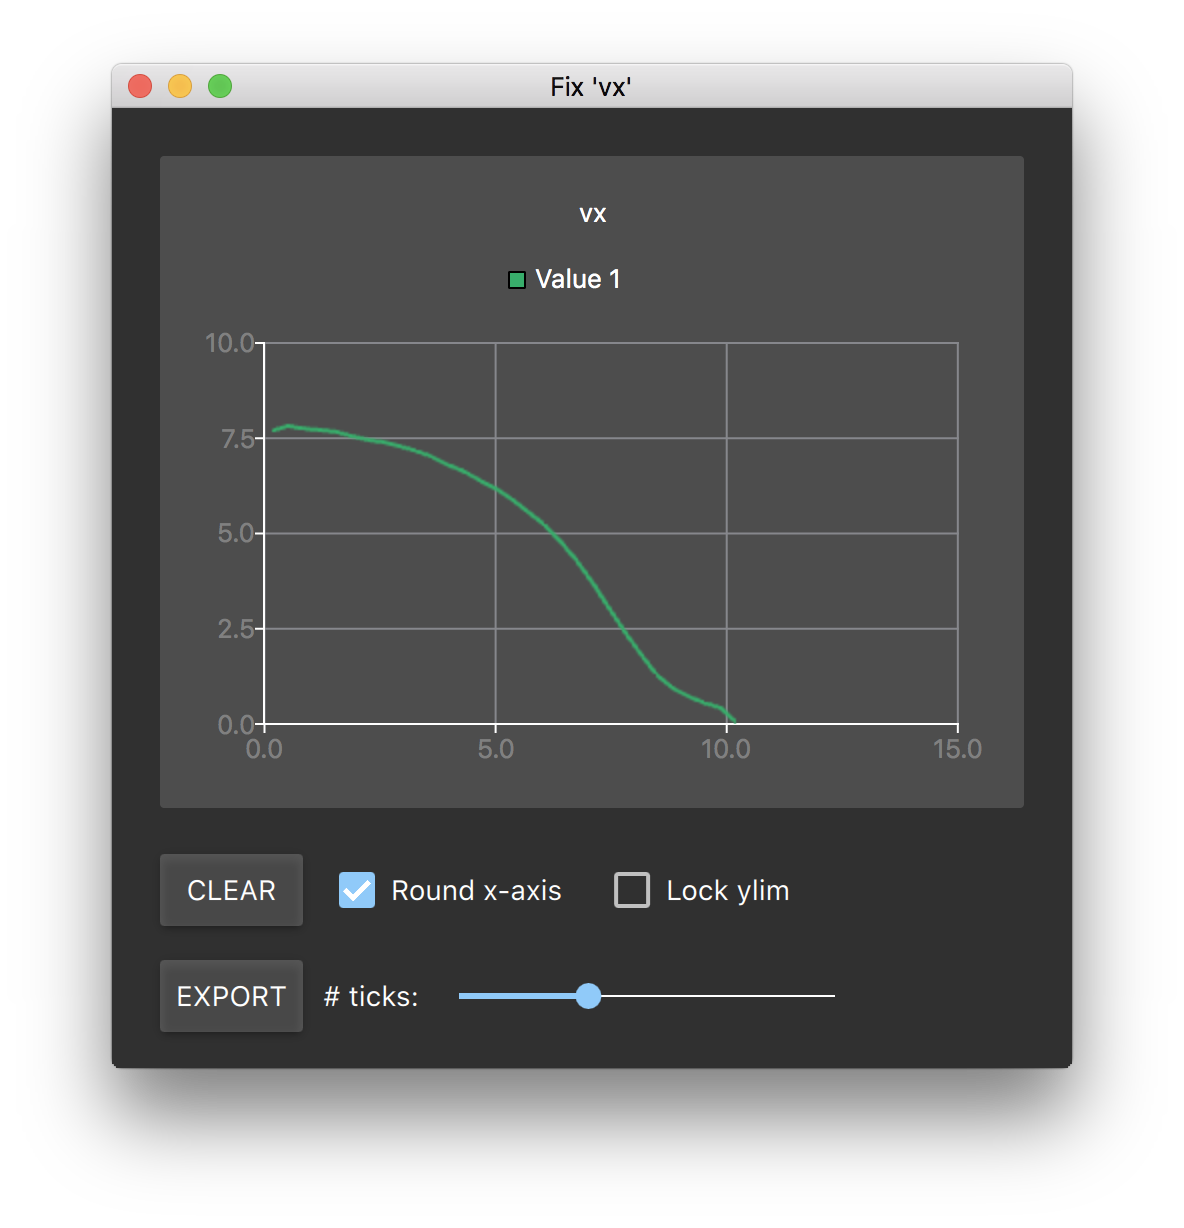
\includegraphics[width=0.5\textwidth]{lj_flow/08_velocity_profile1.png}
	\caption{
		The velocity profile for a Lennard Jones gas inside a nanochannel of radius 8.7 (reduced units).
		Since the wall also is made of Lennard Jones atoms, some of the wall atoms 
		This figure is made using the Atomify real-time plotter which can show any scalar value defined in LAMMPS
		as compute, fix or variable.
    }
	\label{fig:velocity_profile1}
\end{figure}

\subsection{Results}

\begin{figure}
	\centering
	% 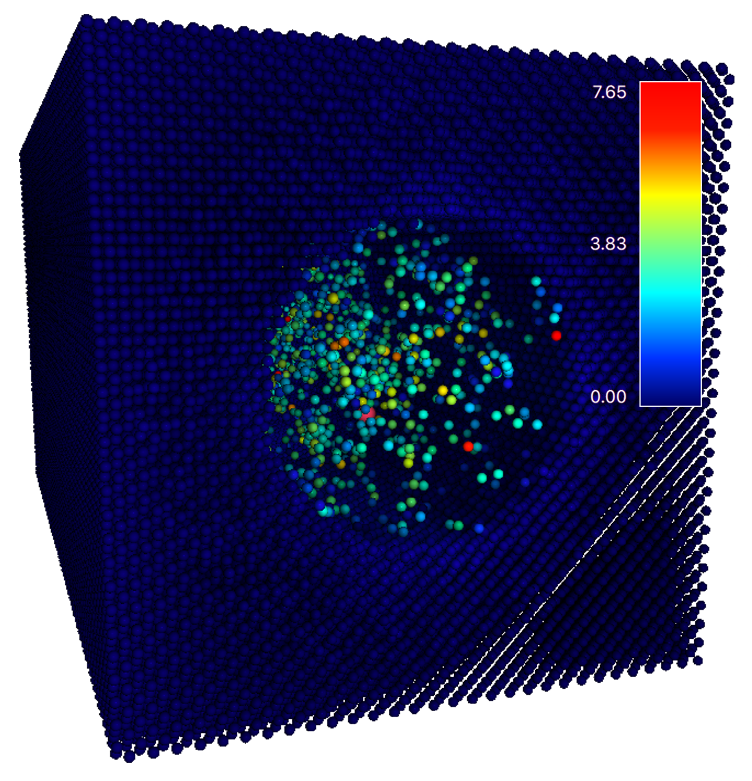
\includegraphics[width=0.5\textwidth]{lj_flow/07_moving.png}
	\caption{
		Velocity profiles for different densities.
		The step flow shape is evident for low density gases with a high non-zero slip velocity.
		When the density increases, the slip velocity goes to zero as expected.
    }
	\label{fig:velocity_profiles}
\end{figure}

We conclude this case study with a series of simulations of the system described above for different densities.
Each simulation runs 10000 timesteps before we export the plots from \code{fix vx} to MATLAB using the Export function seen in Fig. \ref{fig:velocity_profile1}.
All these plots are now merged into a final figure which is shown in Fig. \ref{fig:velocity_profiles}.
It is here evident that the velocity near the boundary is not zero, which is the reason why the permeability is much higher for dilute gases than dense liquids.
As mentioned earlier, this is called the Klinkenberg effect \citep{klinkenberg1941permeability}.

\section{\label{sec:implementation}Implementation}


Atomify runs a LAMMPS instance in the background that it issues commands to.
The current state and atom positions are extracted from this instance for
visualization.
This setup makes it possible for the user to interact with LAMMPS while the
simulation is running.
Atomify is written in C++ and QML using the Qt framework.
The GUI is written in QML, while LAMMPS communication,
computations, and rendering is written in C++.
High-performance visualization is implemented as billboards in Qt3D.

\subsection{Communicating with LAMMPS}

LAMMPS can be compiled as a library with most of its contents being accessable
through either the library interface or public variables in all classes.
LAMMPS provides a C++ API that can be used to access parts of the internal data
in the simulation as well as for issuing commands to LAMMPS.
Further, direct access to raw data in LAMMPS is available through the individual
C++ classes.

\begin{figure}
	\centering
	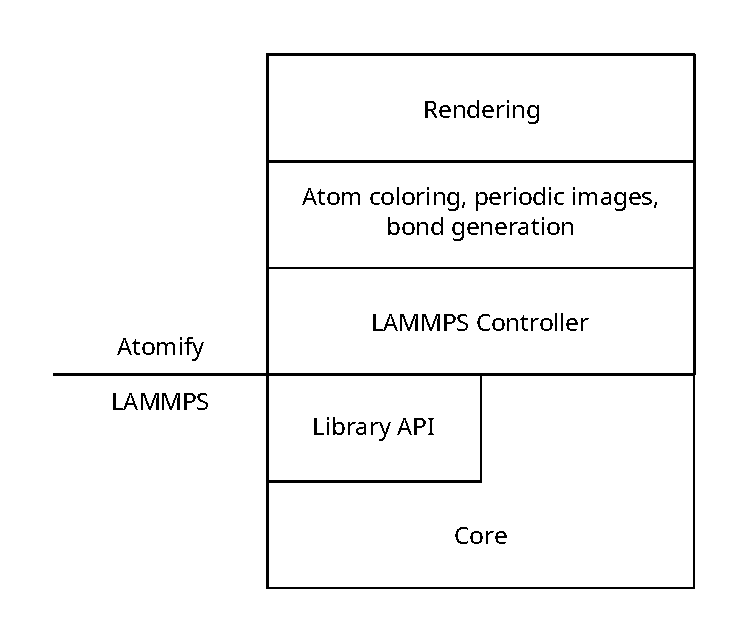
\includegraphics[width=0.5\textwidth]{figures/data-pipeline.pdf}
	\caption{Rendering in Atomify is based on modifying the data from LAMMPS
    by coloring, producing periodic images, and generating bonds between atoms.
    The data is extracted from LAMMPS using the library API and by accessing
    the core classes.}
	\label{fig:data-pipeline}
\end{figure}

The data pipeline from LAMMPS to rendering in Atomify is illustrated in figure
\ref{fig:data-pipeline}.
When rendering one often wants to modify the data from LAMMPS before it is
visualized.
Examples are periodic images of the simulation,
slicing and coloring.
We have been inspired by the pipeline used in Ovito where the data flows through
several \textit{modifiers}, each modifying the visualization data before the
data is converted to a format for the GPU.

\subsection{Rendering techniques}

Simulations of atoms are often visualized using spheres as atoms and cylinders.
The spheres represent the atoms while the cylinders represent the bonds between
the atoms.
This way, the molecular structure is easy to understand and interpret.
In many visualization tools, the spheres and cylinders are built up by many
triangles connected so they form the geometrical object of interest.
One problem with this rendering technique is that each sphere needs many,
often hundreds, of triangles in order to look spherical.
A common technique to overcome this problem is to use billboards.

Billboards are plane objects that are always facing the camera (their normal
vector always points from the billboard center towards the camera center).
Drawing a filled circle on the billboard is a simple approximation to rendering
spheres, but this approach suffers from unrealistic distortions from the field
of view and does not make it possible to render realistic lighting.
The more robust approach, which we have chosen,
is to cast rays from the camera to the plane and calculate the sphere
intersection of each ray.
The normal vector can then be found by subtracting the intersection point from
the sphere center.

The technique of using billboards with only four vertices instead of a mesh
approximating a sphere with many more vertices is often referred to as
\emph{imposter spheres} in the literature.
% TODO add reference to literature explaining the details of rendering spheres with imposter billboards
This technique significantly reduces the number of vertices sent from the CPU to
the GPU, which in turn improves rendering performance.
A sphere may consist of an arbitrary number of vertices,
depending on the level of detail needed.
A billboard will on the other hand consist of only 4 vertices and can be
represented as a point on the CPU which is then expanded on the GPU using shader
programming.
By doing proper shading, the billboards can mimick the spheres and cylinders so
they look realistic, see Fig. \ref{fig:final_billboards}.

\begin{figure}
	\centering
	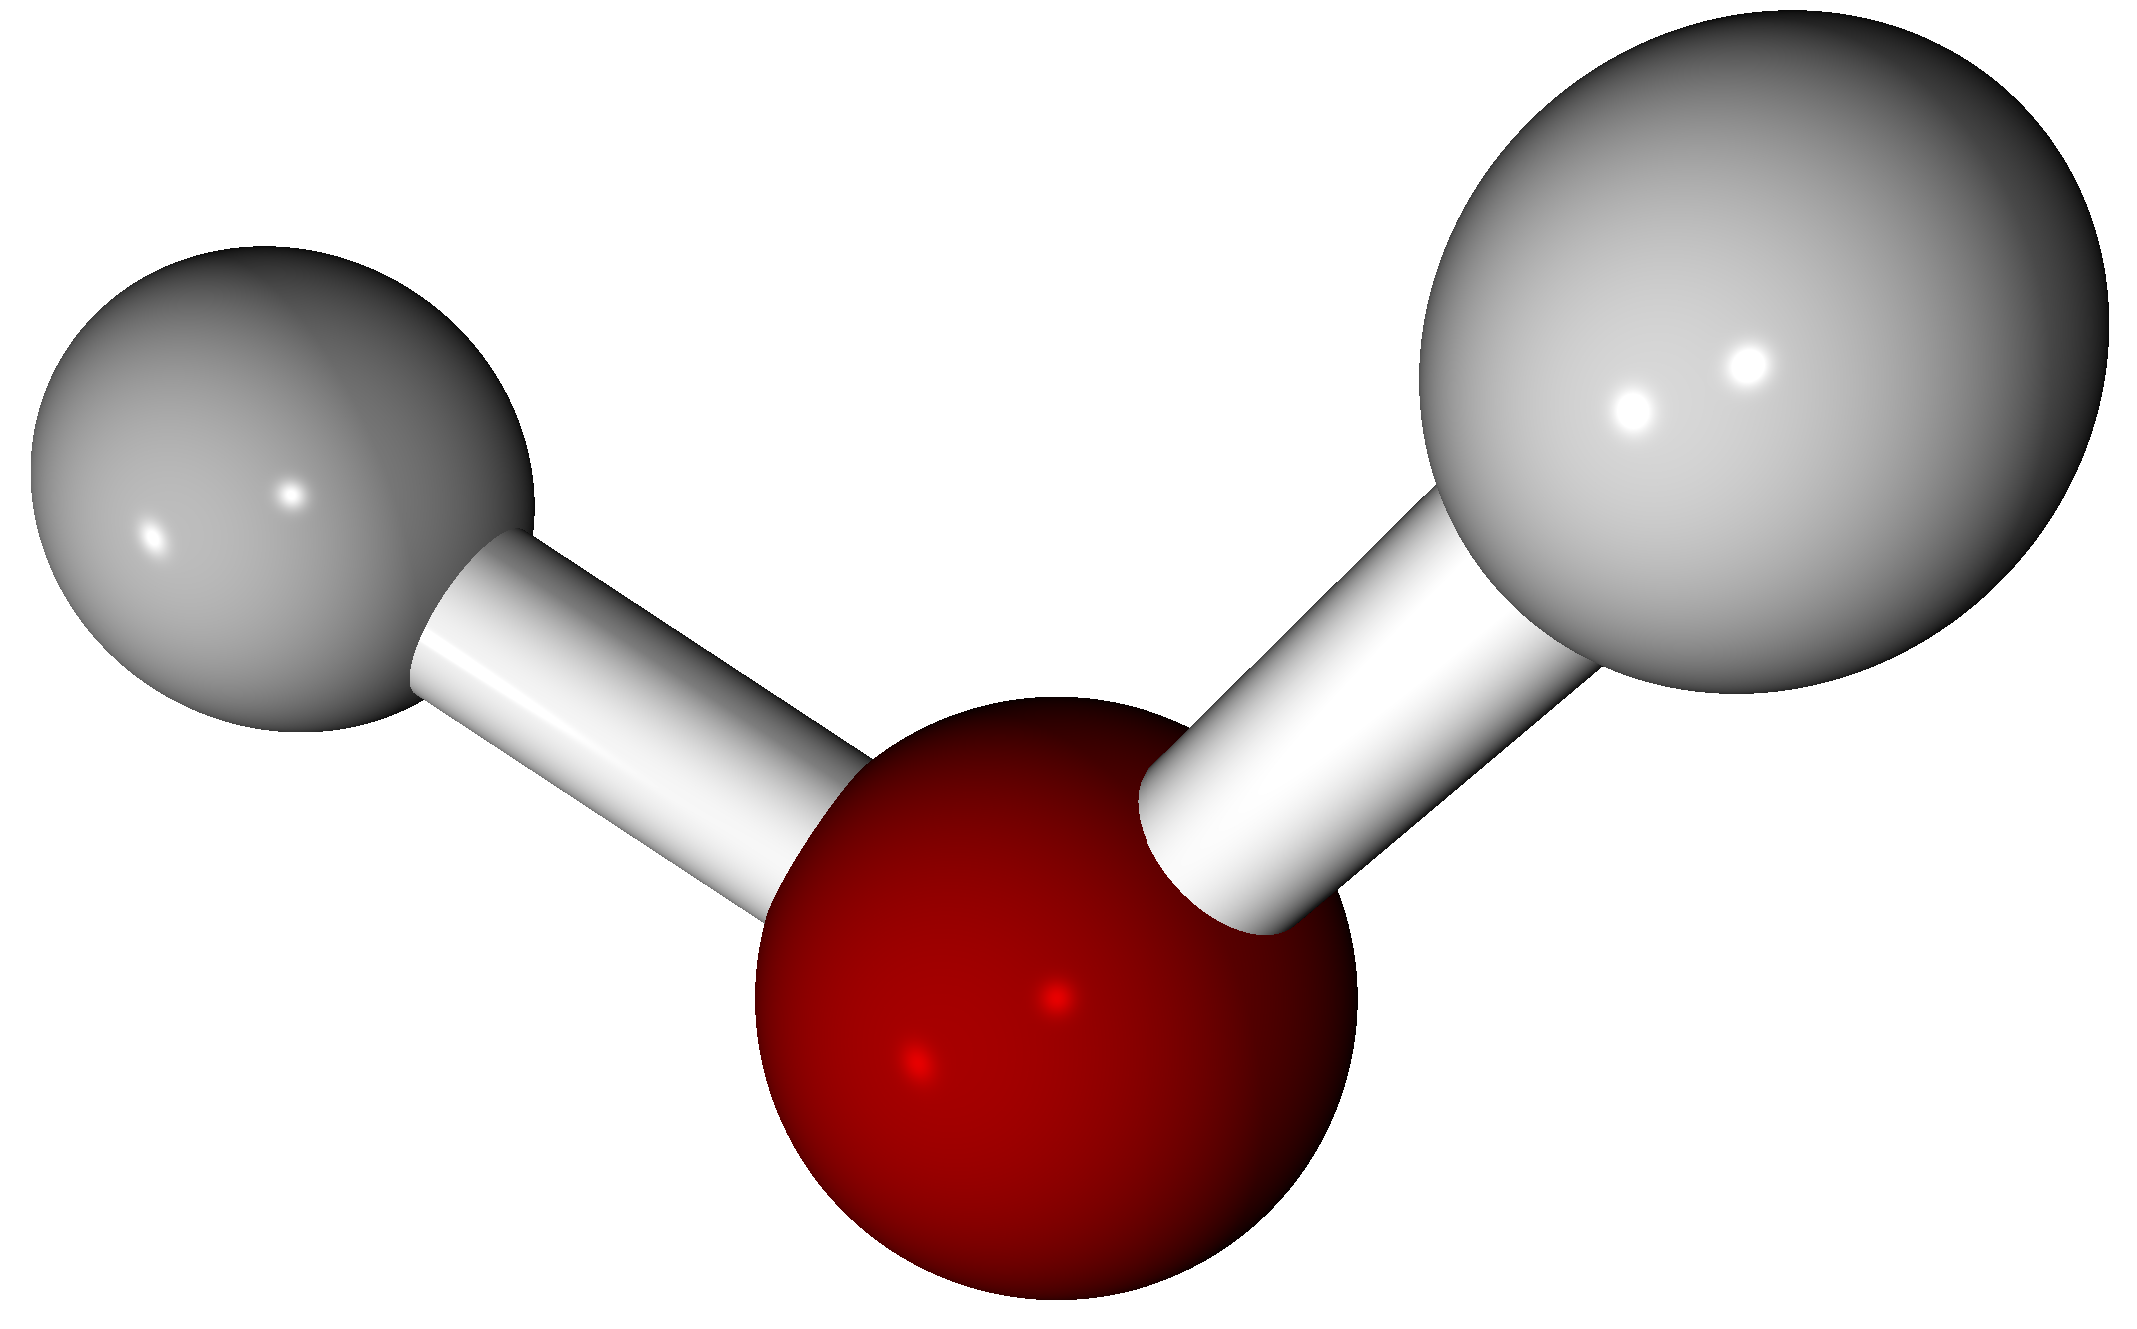
\includegraphics[width=0.5\textwidth]{final_billboard.png}
	\caption{Billboards can produce pixel perfect rendering of molecules. Here we see a water molecule being rendererd with two light sources showing specular reflection and diffuse light effects.}
	\label{fig:final_billboards}
\end{figure}

\subsection{Sphere billboards}

Each sphere is visualized as two triangles making up a square large enough to
cover all pixels the sphere needs.
To reduce the CPU workload, all 4 corner vertices of the square are placed at
the exact position of the sphere.
The radius and a vertex id is specified, so that the vertex shader can move the
4 vertices so that the plane is orthogonal to the view vector and is larger than
the cross sectional area of the sphere of interest.

\subsection{Cylinder billboards}
%
% TODO should we use the other terminology here rather than billboards, something about imposter visualization?
To render bonds in the molecular structure, we have implemented a method that
visualizes realistic cylinder shapes with billboards.
Cylinders are more complicated to visualize with billboards because they have a
more complex geometry.
While spheres obviously are spherically symmetric and can be rendered the same
way regardless of viewing angle, we need to take this into account when
rendering cylinders.
Furhter, the bonds need to intersect with the sphere surface in a way that
needs to be handled by the cylinder rendering technique.

The basic principle is however the same as for the spheres.
We define the vertices needed on the CPU with the same position and add the
necessary information about the cylinder to the vertex attributes.
This information is then used in the vertex shader to draw the triangles of
the billboard.
Finally, ray tracing is used to draw the final cylinder shape based on top
of this billboard.

% TODO mention issue with end caps if this is relevant for the overlapping parts

% TODO explain the details about billboard rendering?

\section{Case study (Anders)}

% TODO Write about case study

\begin{figure}
	\centering
	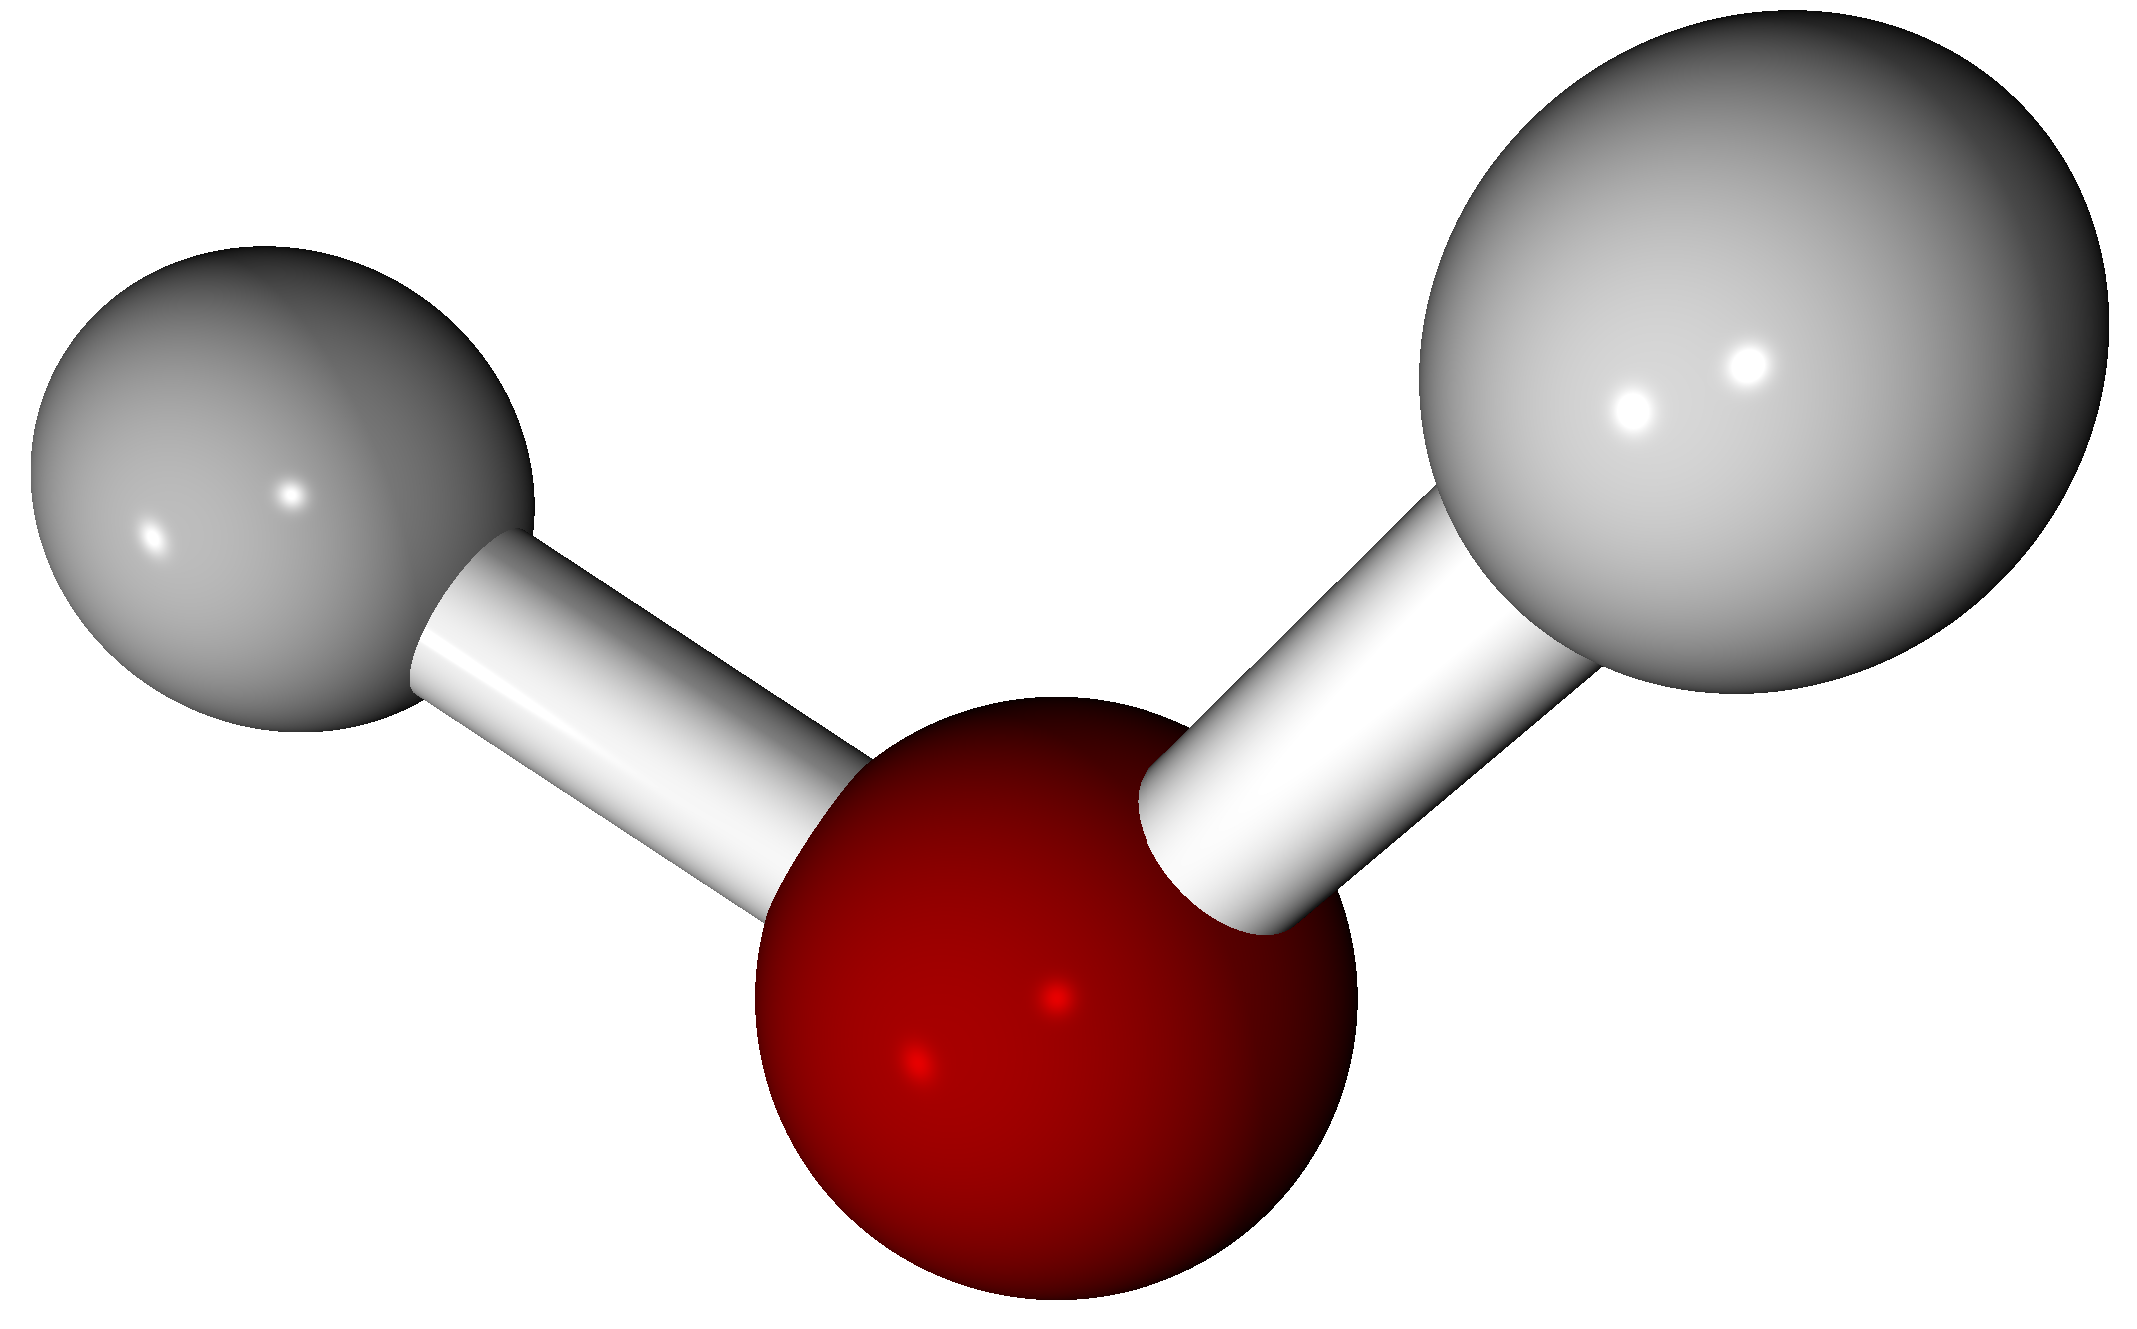
\includegraphics[width=0.5\textwidth]{final_billboard.png}
	\caption{Case study result}
	\label{fig:gui}
\end{figure}

\section{\label{sec:conclusion}Conclusion}
%
We have presented Atomify, a software for live visualization of molecular
dynamics simulations in LAMMPS.
Atomify simplifies the workflow of researchers by combining script development,
analysis and visualization in an intuitive user interface.
The software can also be used to improve training of students using LAMMPS by
providing immediate, visual feedback to script changes.

The simple case study showed how Atomify can be used for quick iteration in 

\section{\label{sec:future}Future work}

Atomify continues in heavy development and we have several features planned for
future versions.
We already have a simple version of Atomify in the web browser using WebGL and WebAssembly.
This makes it easy to test scripts in the browser with all simple functionalities available.
This is especially useful in educational settings where teachers wish to introduce students
to LAMMPS without installing additional software.
It will also serve as a nice demonstration of the full desktop application of
Atomify.

Performance improvements are planned by for instance using geometry shaders in
the rendering pipeline.
This allows a fourfold reduction in the number of vertices passed from the CPU
to the GPU.
Further, geometry shaders can be used for certain modifiers,
such as the periodic copies, which are currently performed on the CPU.

% TODO Reference to KOKKOS
We also aim to include more LAMMPS backends, such as KOKKOS, and running
simulations on computing clusters while visualizing them on the users own
computers.

The script editor will get features such as autocompletion of LAMMPS commands
and easy access to the online documentation by hovering or selecting specific
commands.

We are also working on including Moltemplate and other programs that generate
systems to make it easier for users to get started with more complex
simulations.

\section{Availability}

Atomify is availabe on Linux, MacOS and Windows and can be downloaded from
\href{https://ovilab.net/atomify}{http://ovilab.net/atomify}.
A lightweight version of Atomify is also available for mobile devices running
Android or iOS.

\section{Acknowledgments}

\section{Disclosure}

Svenn-Arne Dragly is employed part-time by The Qt Company.

\bibliography{Remote}

\end{document}
